%%%%%%%%%%%%%%%%%%%%%%% file template.tex %%%%%%%%%%%%%%%%%%%%%%%%%
%
% This is a general template file for the LaTeX package SVJour3
% for Springer journals.          Springer Heidelberg 2010/09/16
%
% Copy it to a new file with a new name and use it as the basis
% for your article. Delete % signs as needed.
%
% This template includes a few options for different layouts and
% content for various journals. Please consult a previous issue of
% your journal as needed.
%
%%%%%%%%%%%%%%%%%%%%%%%%%%%%%%%%%%%%%%%%%%%%%%%%%%%%%%%%%%%%%%%%%%%
%
% First comes an example EPS file -- just ignore it and
% proceed on the \documentclass line
% your LaTeX will extract the file if required
\begin{filecontents*}{example.eps}
    %!PS-Adobe-3.0 EPSF-3.0
    %%BoundingBox: 19 19 221 221
    %%CreationDate: Mon Sep 29 1997
    %%Creator: programmed by hand (JK)
    %%EndComments
    gsave
    newpath
    20 20 moveto
    20 220 lineto
    220 220 lineto
    220 20 lineto
    closepath
    2 setlinewidth
    gsave
    .4 setgray fill
    grestore
    stroke
    grestore
\end{filecontents*}
%
\RequirePackage{fix-cm}
%
%\documentclass{svjour3}                     % onecolumn (standard format)
%\documentclass[smallcondensed]{svjour3}     % onecolumn (ditto)
%\documentclass[smallextended]{svjour3}       % onecolumn (second format)
\documentclass[smallextended,twocolumn]{svjour3}          % twocolumn
%
% FIXME: ADD YOUR FAVOURITE JOURNAL NAME HERE
\journalname{Journal of Reproducible Research}
\smartqed  % flush right qed marks, e.g. at end of proof
\usepackage{graphicx}
%usepackage{mathptmx}      % use Times fonts if available on your TeX system
\usepackage{natbib}


\usepackage{amsmath}
\usepackage{textcomp}
\usepackage{booktabs}
\usepackage{units}
\usepackage{hyperref}
\usepackage{wrapfig}
%\usepackage{todonotes}
\usepackage{csvsimple}

%%%%%%%%%%%%%%%%%%%%%%%%%%%%%%%%%%%%%%%%%%%%%%%%%%%%%%%%%%%%%%%%%%%

\begin{document}

% This file contains variable definitions with results
\newcommand{\SetosaPrecision}{1.00}
\newcommand{\SetosaRecall}{1.00}
\newcommand{\SetosaF}{1.00}
\newcommand{\SetosaSupport}{7.00}
\newcommand{\VersicolorPrecision}{0.85}
\newcommand{\VersicolorRecall}{0.92}
\newcommand{\VersicolorF}{0.88}
\newcommand{\VersicolorSupport}{12.00}
\newcommand{\VirginicaPrecision}{0.90}
\newcommand{\VirginicaRecall}{0.82}
\newcommand{\VirginicaF}{0.86}
\newcommand{\VirginicaSupport}{11.00}
\newcommand{\MAPrecision}{0.92}
\newcommand{\MARecall}{0.91}
\newcommand{\MAF}{0.91}
\newcommand{\MASupport}{30.00}
\newcommand{\WAPrecision}{0.90}
\newcommand{\WARecall}{0.90}
\newcommand{\WAF}{0.90}
\newcommand{\WASupport}{30.00}
\newcommand{\accuracy}{0.9}


\onecolumn
% FIXME: ADD YOUR TITLE HERE
\title{Writing a reproducible paper}

% FIXME: ADD YOURSELF AS AN AUTHOR
\author{%
  Alice~Allison \and Bob~McBobFace\\}
% FIXME: ADD NAME AND AFFILIATION
\institute{Alice~Allison \at
Max Planck Institute for Human Development, Institute for Open Science, Lentzallee 94, Berlin, Germany
\email{first.last@gmail.com}
%Tel.: +123-45-678910\\
%Fax: +123-45-678910\\
%\email{fauthor@example.com}           %  \\
%             \emph{Present address:} of F. Author  %  if needed
\and
Bob~McBobFace \at
Research Centre Juelich, Institute for Reproducible Research, Juelich Germany
\email{first.last@gmail.com}
}

\date{Received: date / Accepted: date}

\maketitle

% Please list all authors that played a significant role in the research
% involved in the article. Please provide full affiliation information
% (including full institutional address, ZIP code and e-mail address) for all
% authors, and identify who is/are the corresponding author(s).

%%%%%%%%%%%%%%%%%%%%%%%%%%%%%%%%%%%%%%%%%%%%%%%%%%%%%%%%%%%%%%%%%%%

\begin{abstract}

% Abstracts should be up to 300 words and provide a succinct summary of the
% article. Although the abstract should explain why the article might be
% interesting, care should be taken not to inappropriately over-emphasize the
% importance of the work described in the article. Citations should not be used
% in the abstract, and the use of abbreviations should be minimized. If you are
% writing a Research or Systematic Review article, please structure your
% abstract into Background, Methods, Results, and Conclusions.

There are many tools that make it not only possible, but also easy to create reproducible research.
It is often not straightforward to know, however, which tools are available, how
they are to be used, and how they can interoperate with eachother, if necessary.
This paper demonstrates \textit{one way} of using \textit{one set} of tools (Git,
DataLad, \LaTeX\, and Make/Makefiles) interoperably to create a dynamically generated,
automatically reproducible research object.
In this example, DataLad is used to link code, manuscript, and data.
Within a Python script that computes results and figures, DataLad's Python API is used
to retrieve data automatically.
The \LaTeX\ manuscript does not hard-code results or tables, but embeds external
files or variables with results.
The Python script saves its results and figures into the dataset, but also outputs
results in form that they can be embedded into the manuscript as variables.
To orchestrate code execution and \LaTeX\ manuscript compiling, a Makefile is
used.
With this setup, generating a manuscript with freshly computed results is a matter
of running \texttt{make} in a cloned repository.

\keywords{%
open science \and
reproducible research \and
dynamic document generation \and
open source software
}
\end{abstract}

%\todo[inline]{Here is a todo note}

%%%%%%%%%%%%%%%%%%%%%%%%%%%%%%%%%%%%%%%%%%%%%%%%%%%%%%%%%%%%%%%%%%%

\twocolumn
\section*{Introduction}\label{intro}


Many tools, workflows and tutorials exist or are being developed to make
reproducible science "too easy not to do" \citep{the_turing_way}, e.g. \citet{van2020worcs}
or \cite{peikert_brandmaier_2019}.
The greatest hurdle to using those tools or workflows is in many cases getting to
know about them.
This small example paper is a demonstration of using the tools Git, DataLad, Make,
Python, and \LaTeX\ in conjunction to create a dynamically generated document.
This is by no means the only way to generate such a document, and certainly not the
easiest, but it a demonstration of \textit{one} way of doing it.

It also does not use all features and capabilities of DataLad, but uses it "only"
to link all relevant workflow elements together into a domain agnostic, common data
structure as the basis for decentralized research data management (RDM).


\section*{Methods}\label{methods}

We use DataLad to package all relevant aspects to create an open and transparent
digital research object into a domain agnostic, common data structure, the DataLad
dataset.
This dataset allows for decentralized research data management, a concept that is
visualized in Figure \ref{fig:RDM}.
%
\subsection*{Operation}\label{op}

Since the repository is a DataLad dataset that includes input data as a subdataset
and a script that retrieves data prior to result computation, and given that a
Makefile handles the execution of all relevant commands in the correct order, the
only necessary command to generate this manuscript after cloning it from a repository
hosting site is

%
\begin{verbatim}
make
\end{verbatim}
%

\subsection*{Analysis}

As an example, this repository performs the analysis that is demonstrated in
\href{http://handbook.datalad.org/en/latest/basics/101-130-yodaproject.html}{this section of the DataLad Handbook}
\citep{handbook}:
A K-Nearest-Neighbour Classification analysis on a standard tutorial dataset.
The dataset is the Iris dataset, a small dataset commonly used for introductory
machine-learning tutorials.
It consists of measurements of sepal and petal length and width from three
different species of iris flowers, Virginica, Setosa, and Versicolor.

\begin{figure}
  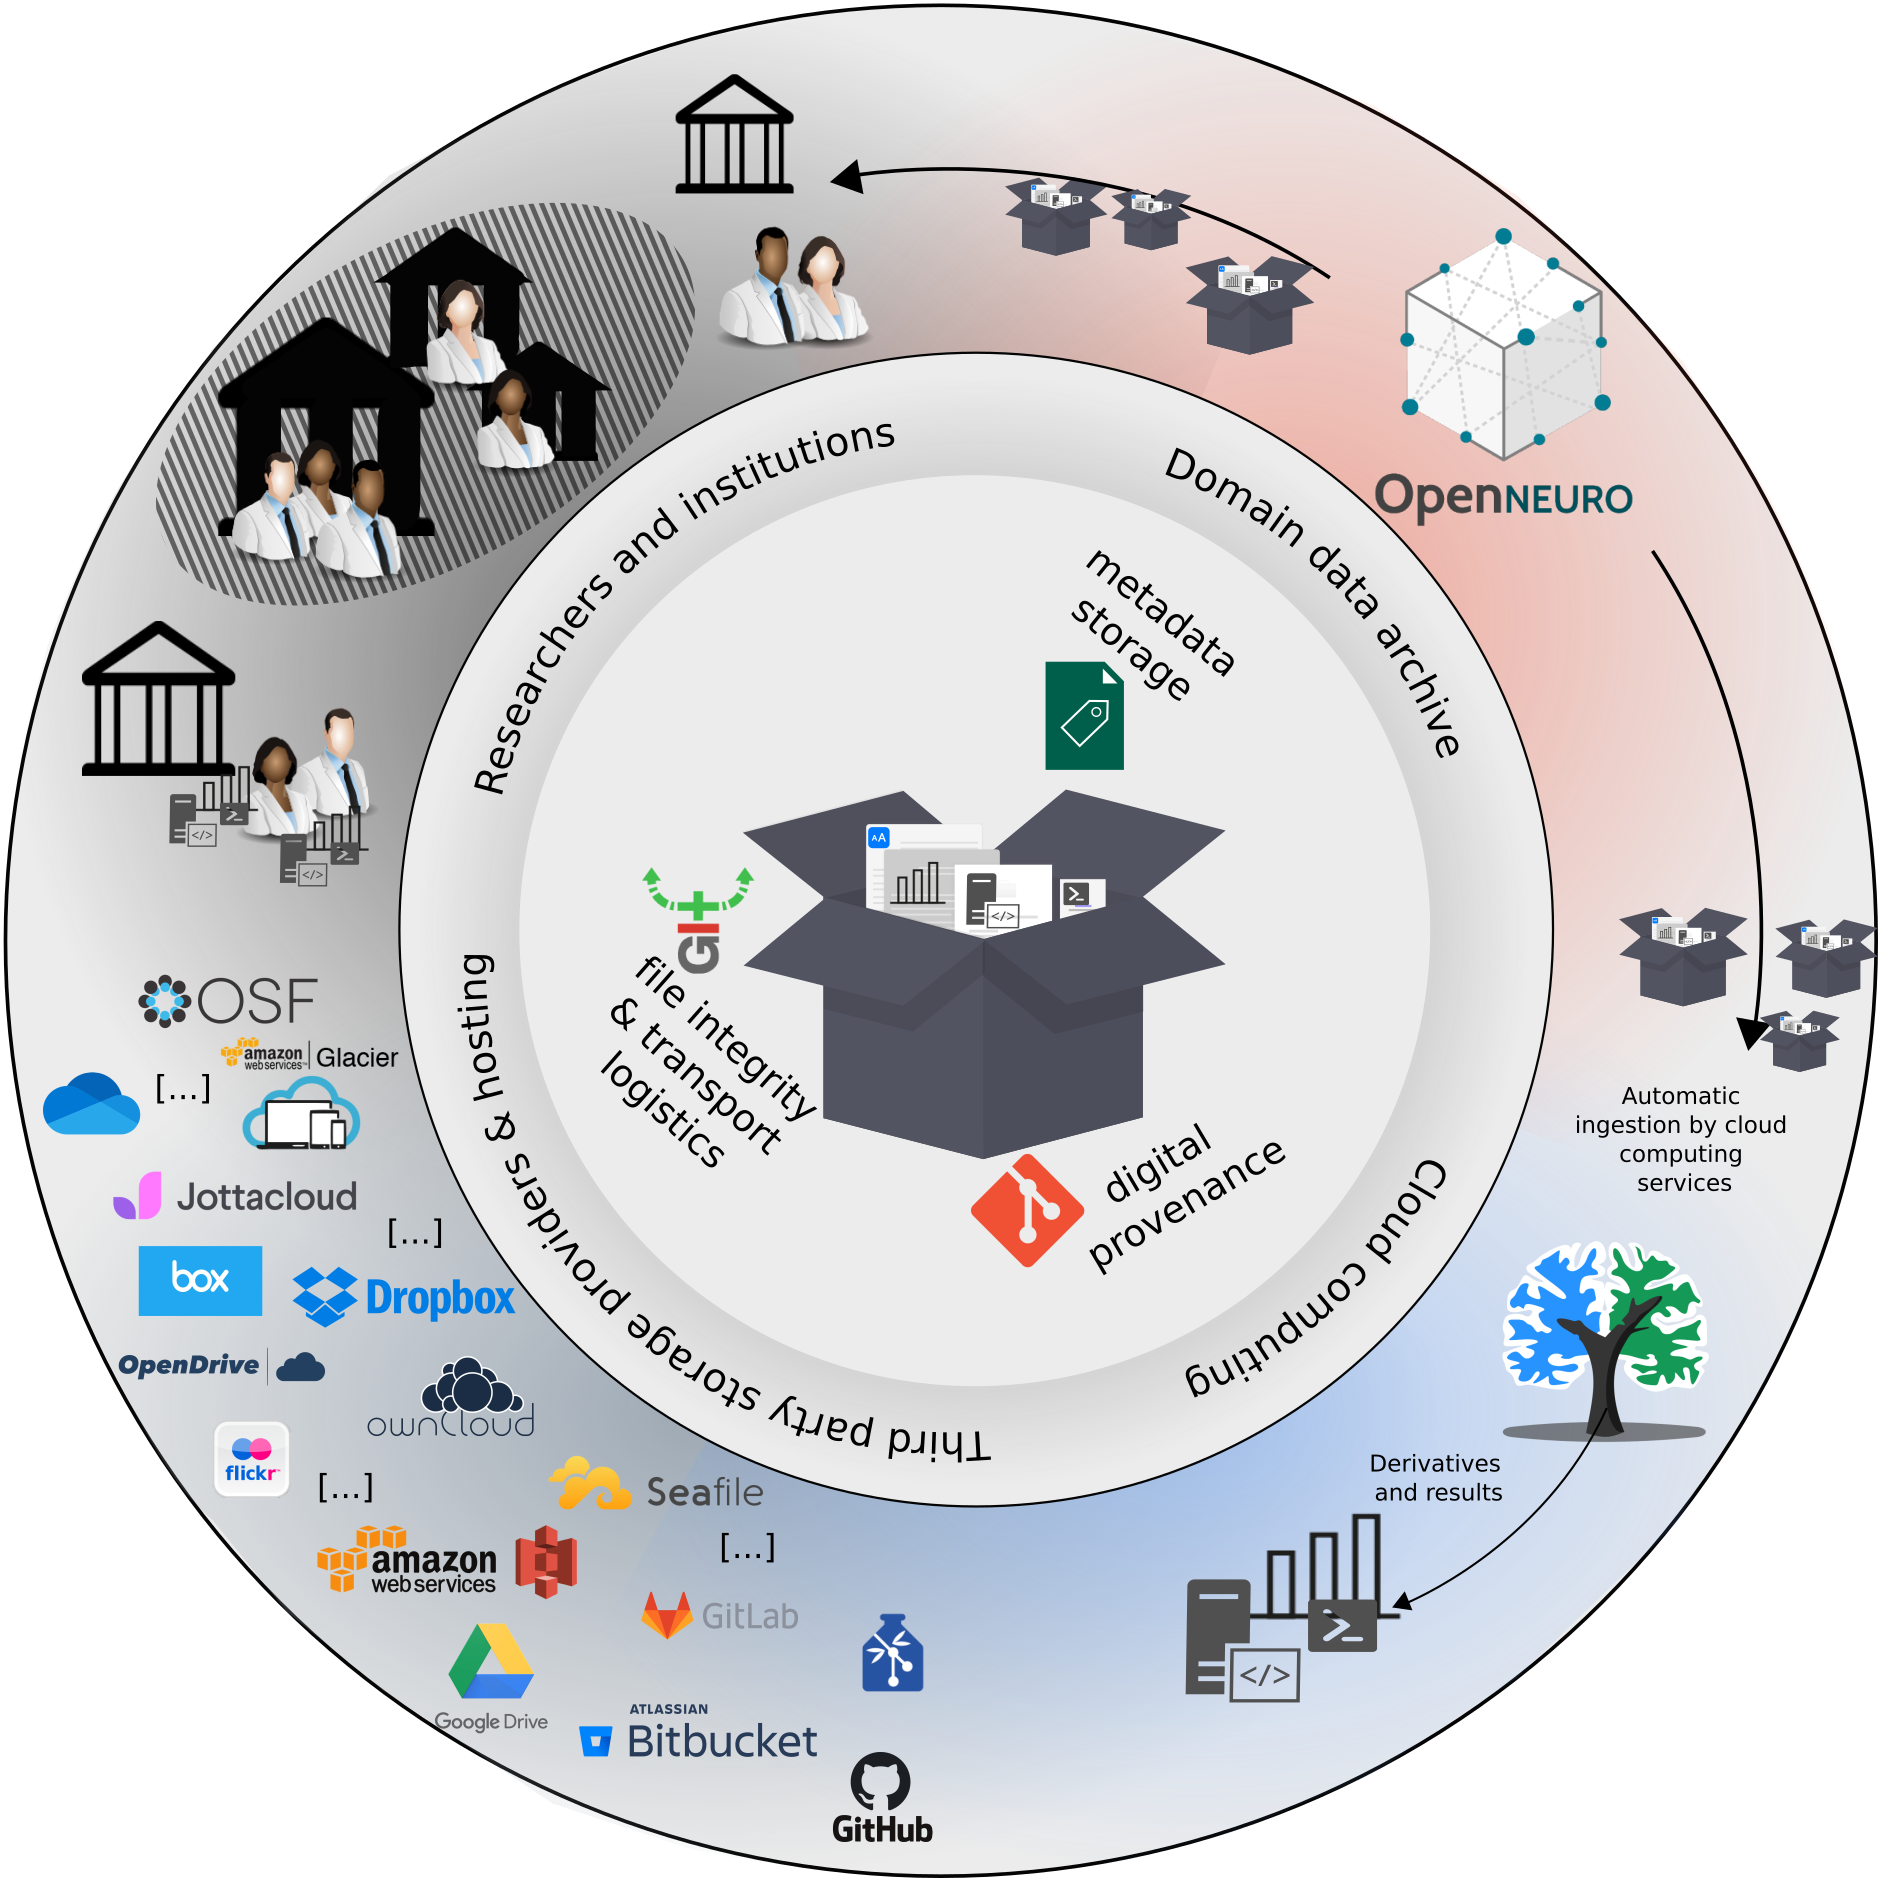
\includegraphics[trim=0 0 0 0,clip,width=0.5\textwidth]{img/decentral_RDM_overview.png}
  \caption{A DataLad dataset is a domain agnostic data structure that can serve as
  a basis for decentralized data management.
  A dataset can include and share any digital research object and its provenance,
  and interfaces with a vast amount of third party storage and hosting providers.}
  \label{fig:RDM}
\end{figure}



\section*{Results}\label{res}

%
Figure \ref{fig:relation} shows the pairwise relationships between the variables in the dataset.
This figure is created by a script and embedded into the manuscript during \texttt{make}.

\begin{figure}
  \includegraphics[width=0.5\textwidth]{img/pairwise_relationships.png} \\
  % figure caption is below the figure
  \caption{Pairwise relationships in the iris dataset.}
  % Give a unique label
  \label{fig:relation}
\end{figure}

The overall accuracy of the prediction is \accuracy.
The complete prediction report of the classification, split by flower species
and including the weighted average and the macro average, is displayed in
Table \ref{tab:predictions}.

% create a table with custom variables
\begin{table}
  % table caption is above the table
    \caption{Prediction metrics embedded as LaTeX variables}
        % Give a unique label
        \label{tab:predictions}
         % For LaTeX tables use
        \begin{tabular}{|c|llll|}
        \hline
                            & \textbf{precision}   & \textbf{recall}   & \textbf{f1-score} & \textbf{support}   \\
        \hline
            Setosa          & \SetosaPrecision     & \SetosaRecall     & \SetosaF          & \SetosaSupport     \\
            Versicolor      & \VersicolorPrecision & \VersicolorRecall & \VersicolorF      & \VersicolorSupport \\
            Virginica       & \VirginicaPrecision  & \VirginicaRecall  & \VirginicaF       & \VirginicaSupport  \\
        \hline
            macro avg       & \MAPrecision         & \MARecall         & \MAF              & \MASupport         \\
            weighted avg    & \WAPrecision         & \WARecall         & \WAF              & \WASupport         \\
        \hline
  \end{tabular}
\end{table}

Table \ref{tab:predictions} was created with custom variable definitions.
Its is, however, equally possible to simply embed a CSV file as a table, which has
been done with the result file \texttt{prediction\_report.csv} in Table \ref{tab:predictions2}.

% embed a table from a csv file
\begin{table}
  % table caption is above the table
    \caption{Prediction metrics as imported from csv file}
        \label{tab:predictions2}
        \begin{tabular}{cllll}
            \csvautotabular{prediction_report.csv}
        \end{tabular}
\end{table}

\section*{Conclusion}\label{con}

In order to achieve transparent, reproducible, and open science, a manuscript
should entail more than only a PDF, but contain all relevant elements to rerun
an analysis and reproduce a result.
There are many ways to do so, and this is one of them.
%
Note that this demonstration is vastly simplified.
A published paper as a complex real-world example can be found at \\
\href{https://github.com/psychoinformatics-de/paper-remodnav/}{github.com/psychoinformatics-de/paper-remodnav/}.


\begin{acknowledgements}

Open Science stands on the shoulder of giants: Open Source Software tools.
Cite the tools you use. :)

\end{acknowledgements}

\bibliographystyle{spbasic}      % basic style, author-year citations
\bibliography{references}

% References can be listed in any standard referencing style that uses a numbering system
% (i.e. not Harvard referencing style), and should be consistent between references within
% a given article.

% Reference management systems such as Zotero provide options for exporting
% bibliographies as Bib\TeX{} files. Bib\TeX{} is a bibliographic tool that is
% used with \LaTeX{} to help organize the user's references and create a
% bibliography. This template contains an example of such a file,
% \texttt{sample.bib}, which can be replaced with your own. Use the
% \verb|\cite| command  to create in-text citations, like this
% \cite{Smith:2012qr} and this \cite{Smith:2013jd}.

\clearpage

\end{document}
